
\subsection{SDN}

%
% SDN
%
\begin{frame}\frametitle{SDN}

    \begin{itemize}
    \item Software Defined Networking (Redes definidas por software)
    \end{itemize}
        \begin{figure}[h]
        \centering
        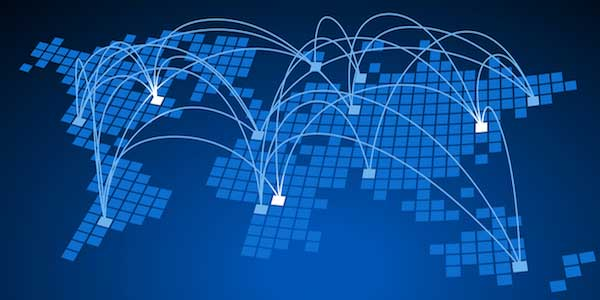
\includegraphics[scale=0.5]{images/sdn.jpg}
    \end{figure}
\end{frame}


%
% SDN
%
\begin{frame}\frametitle{SDN}

    \begin{itemize}
    \item Separa o plano de \emph{dados} do plano de \emph{controle}
    \end{itemize}
        \begin{figure}[h]
        \centering
        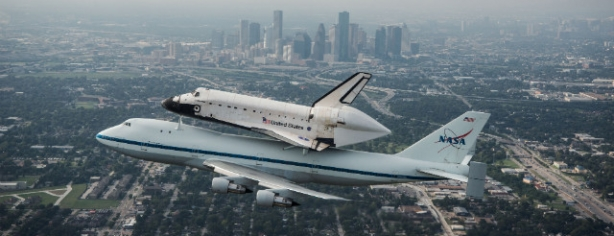
\includegraphics[scale=0.5]{images/planes.jpg}
    \end{figure}
\end{frame}


%
% Data plane
%
\begin{frame}\frametitle{Data Plane}

    \begin{itemize}
    \item Encaminhamento de pacotes
    \item Comutação no \emph{hardware} do \emph{switch}
    \end{itemize}
        \begin{figure}[h]
        \centering
        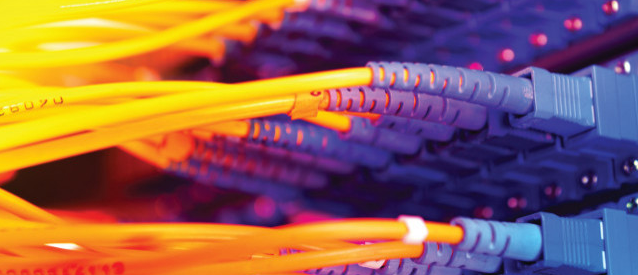
\includegraphics[scale=2.0]{images/data-plane.png}
    \end{figure}
\end{frame}


%
% Control plane
%
\begin{frame}\frametitle{Control Plane}

    \begin{itemize}
    \item Decidir como encaminhar os pacotes
    \item Roteamento, políticas e visão topológica
    \end{itemize}
        \begin{figure}[h]
        \centering
        
\includegraphics[scale=0.5]{images/control-plane.png}
    \end{figure}
\end{frame}




%
% SDN
%
\begin{frame}\frametitle{SDN}

    \begin{itemize}
    \item SDN é apenas um modelo
    \vspace*{0.5cm}
    \item Um \emph{design} para construção e administração de redes
    \vspace*{0.5cm}
    \item A separação dos planos de controle e de dados torna o 
          funcionamento da rede mais flexível
    \end{itemize}
\end{frame}

%
% SDN
%
\begin{frame}\frametitle{Características}

    \begin{itemize}
    \item Torna a rede programável
    \vspace*{0.1cm}
    \item Flexibilidade na administração da rede
    \vspace*{0.1cm}
    \item Controle logicamente centralizado
    \vspace*{0.1cm}
    \item Configurável via programação
    \vspace*{0.1cm}
    \item Padronização aberta 
    \end{itemize}
\end{frame}

